\documentclass[12pt,letterpaper]{article}
\usepackage[utf8]{inputenc}
\usepackage[spanish]{babel}
\usepackage{graphicx}
\usepackage[left=2cm,right=2cm,top=2cm,bottom=2cm]{geometry}
\usepackage{graphicx} % figuras
% \usepackage{subfigure} % subfiguras
\usepackage{float} % para usar [H]
\usepackage{amsmath}
%\usepackage{txfonts}
\usepackage{stackrel} 
\usepackage{multirow}
\usepackage{enumerate} % enumerados
\renewcommand{\labelitemi}{$-$}
\renewcommand{\labelitemii}{$\cdot$}


% \author{}
% \title{Caratula}
\begin{document}

% Fancy Header and Footer
% \usepackage{fancyhdr}
% \pagestyle{fancy}
% \cfoot{}
% \rfoot{\thepage}
%

% \usepackage[hidelinks]{hyperref} % CREA HYPERVINCULOS EN INDICE

% \author{}
\title{Caratula}

\begin{titlepage}
\begin{center}
\large{UNIVERSIDAD PRIVADA DE TACNA}\\
\vspace*{-0.025in}
\begin{figure}[htb]
\begin{center}

\includegraphics[width=8cm]{./Imagenes/logo}
\end{center}
\end{figure}
\vspace*{0.15in}
INGENIERÍA DE SISTEMAS  \\

\vspace*{0.5in}
\begin{large}
TITULO:\\
\end{large}

\vspace*{0.1in}
\begin{Large}
\textbf{Informe de laboratorio 01} \\
\end{Large}

\vspace*{0.3in}
\begin{Large}
\textbf{CURSO:} \\
\end{Large}

\vspace*{0.1in}
\begin{large}
Calidad y Pruebas de Software\\
\end{large}

\vspace*{0.3in}
\begin{Large}
\textbf{DOCENTE(ING):} \\
\end{Large}

\vspace*{0.1in}
\begin{large}
 Patrick Cuadros Quiroga\\
\end{large}

\vspace*{0.2in}
\vspace*{0.1in}
\begin{large}
Integrante: \\
\begin{flushleft}
Percy Taquila Carazas\hfill	(2018061088) \\
\end{flushleft}
\end{large}
\end{center}

\end{titlepage}

\tableofcontents % INDICE
\thispagestyle{empty} % INDICE SIN NUMERO
\newpage
\setcounter{page}{1} % REINICIAR CONTADOR DE PAGINAS DESPUES DEL INDICE


\section{Objetivos} 

- Implementar SonarQube para pruebas de calidad.


\section{Requerimientos} 

\begin{itemize}
\item Windows Education 10
\item  SonarQube
\item Docker Desktop
\end{itemize}



\section{Desarrollo}

\textbf{1.Descargar SonarQube}

    \begin{center}
		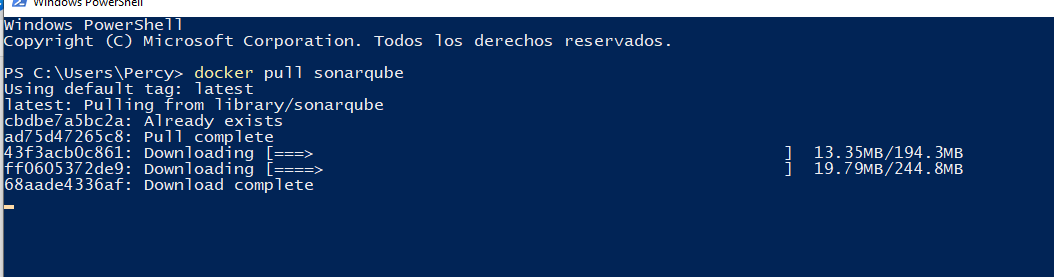
\includegraphics[width=15cm]{./Imagenes/1} 
	\end{center}

\textbf{2. Ejecutar una instancia de SonarQube}

    \begin{center}
		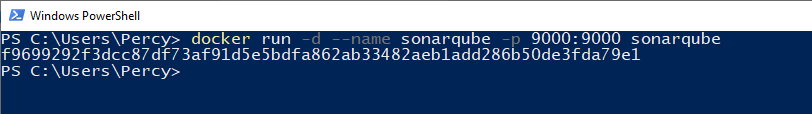
\includegraphics[width=15cm]{./Imagenes/2} 
	\end{center}
  
  
\textbf{3.Ingresar al portal con las credenciales}

    \begin{center}
		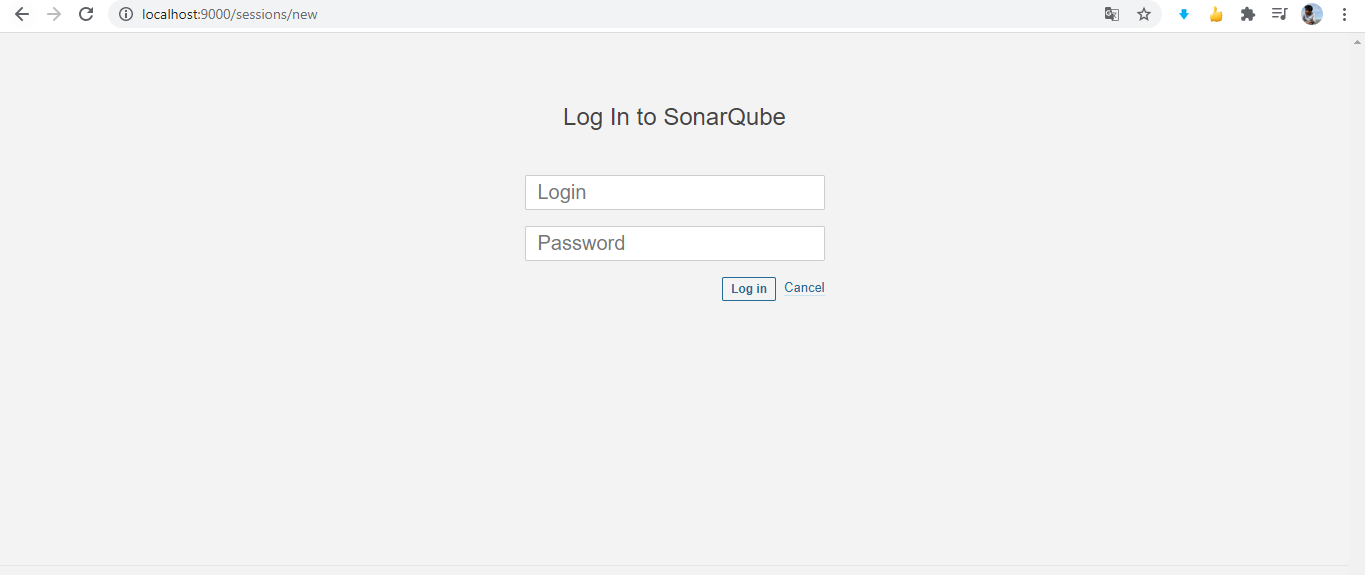
\includegraphics[width=15cm]{./Imagenes/3} 
	\end{center}

\textbf{4. Crear una nueva aplicación con el nombre aplicacionNetCore}

    \begin{center}
		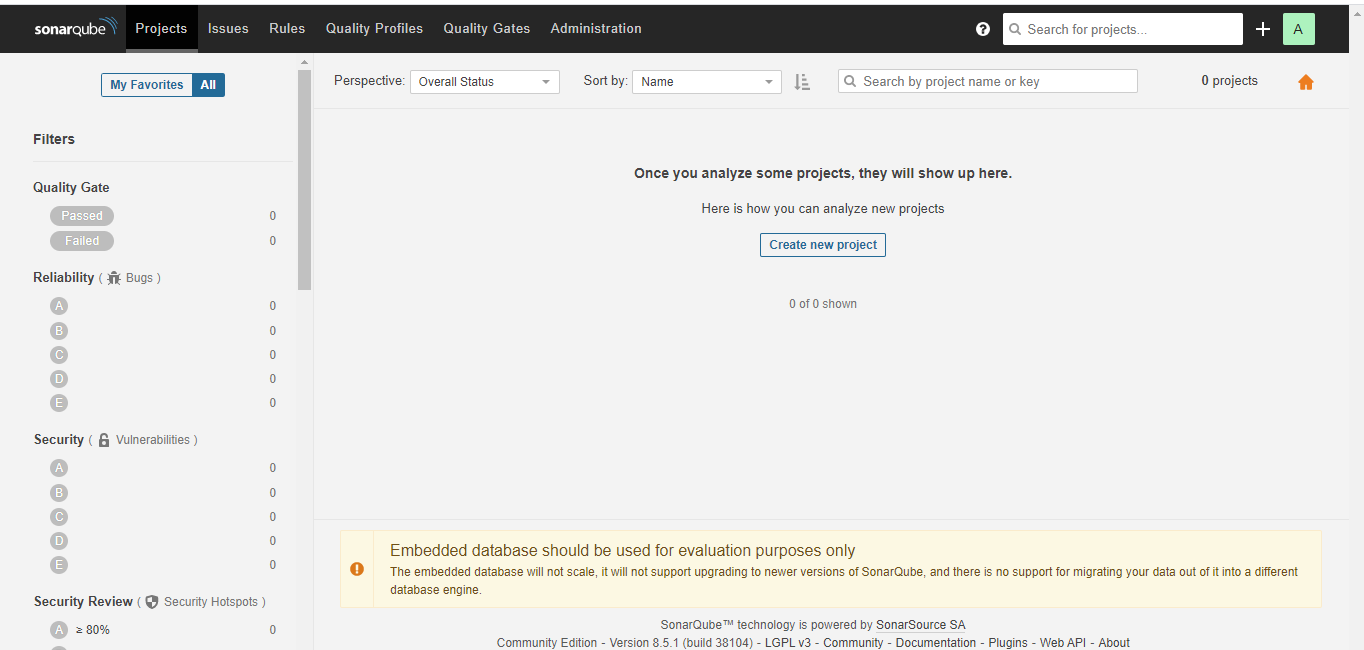
\includegraphics[width=15cm]{./Imagenes/4} 
	\end{center}
	
	 \begin{center}
		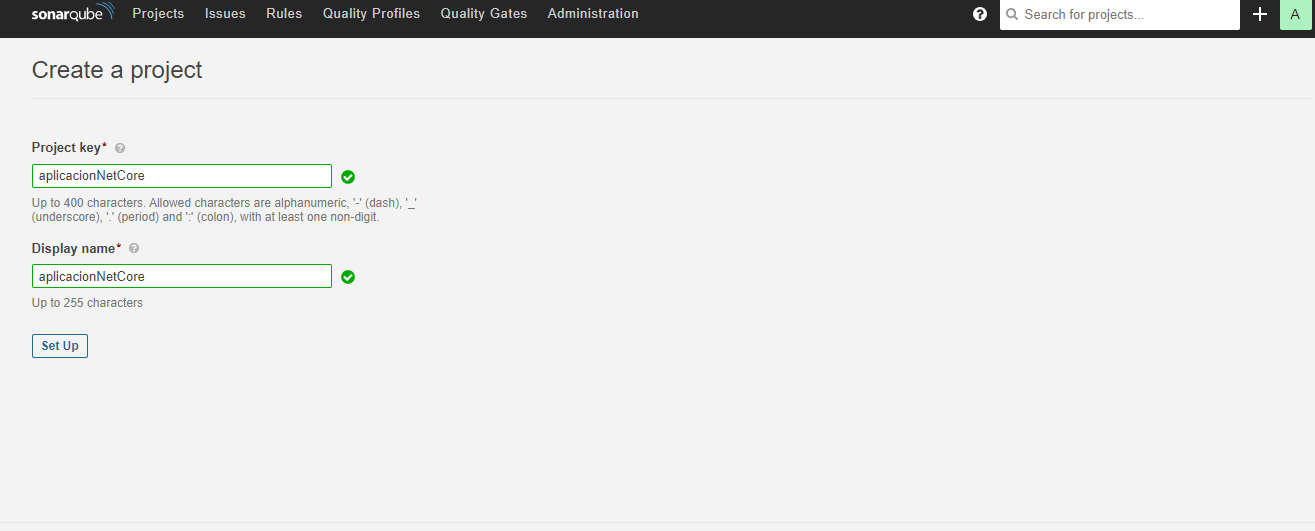
\includegraphics[width=15cm]{./Imagenes/5} 
	\end{center}


\textbf{5.Generar el token de la nueva aplicación aplicacionNetCore, debera devolver algo similar a 8a15d2a89c8636f15eb32ebee0993b8d16bff94e}

    \begin{center}
		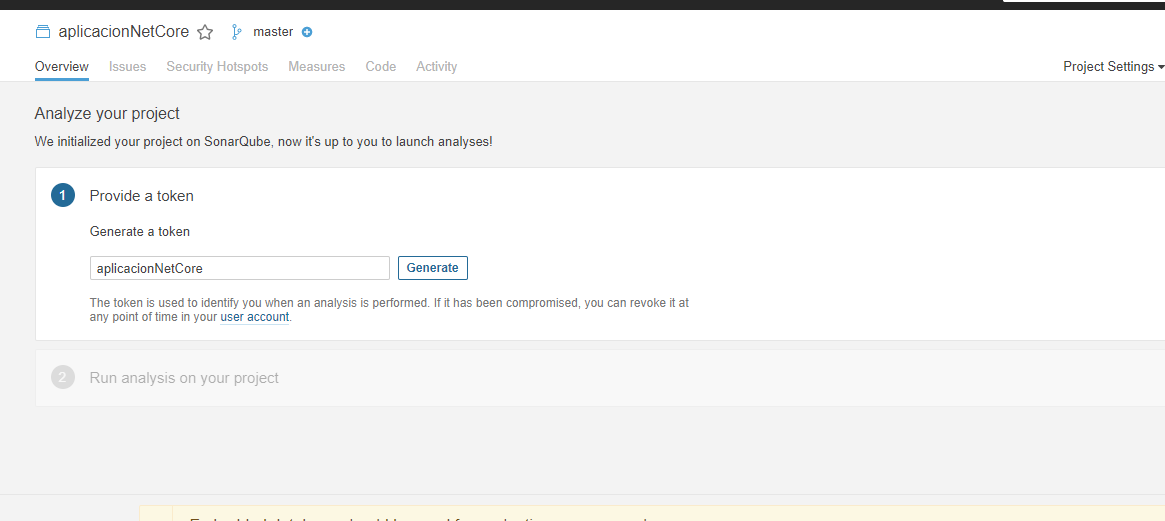
\includegraphics[width=15cm]{./Imagenes/6} 
	\end{center}
	
	 \begin{center}
		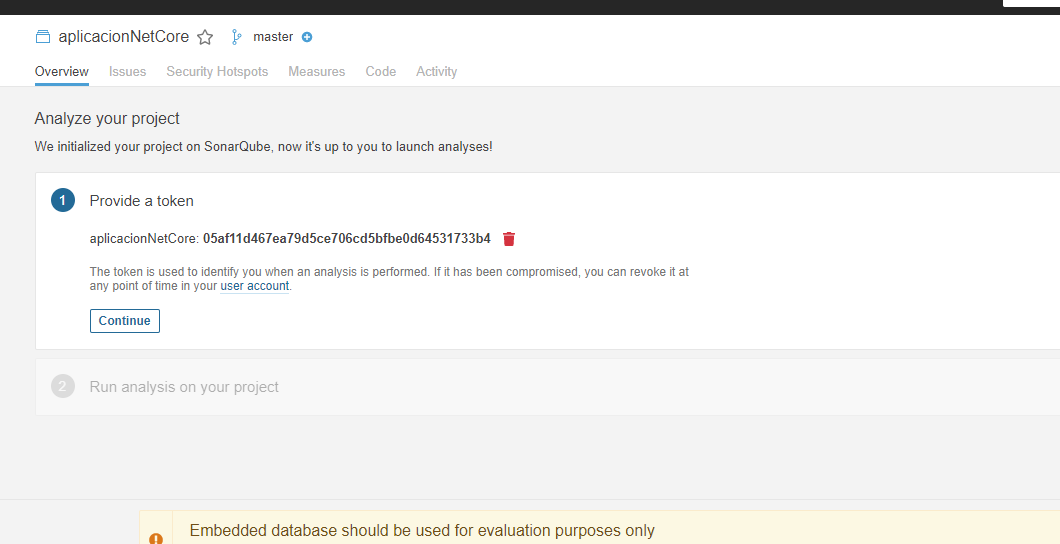
\includegraphics[width=15cm]{./Imagenes/7} 
	\end{center}


\textbf{6. Descargar Net Core e instalar}

    \begin{center}
		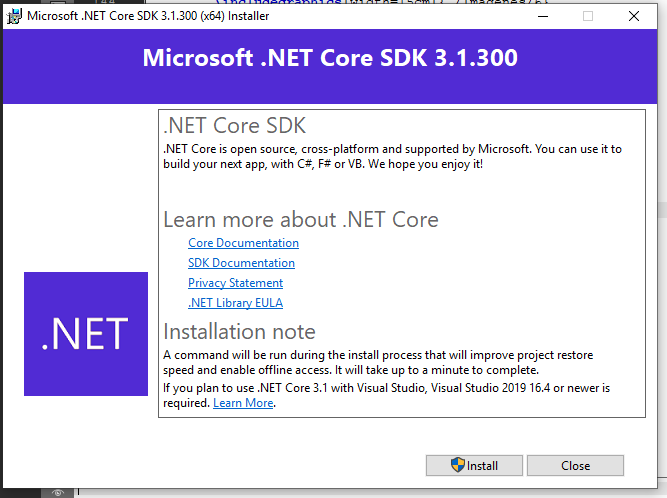
\includegraphics[width=15cm]{./Imagenes/8} 
	\end{center}

\textbf{7. En un terminal ejecutar e instalar sonar-scanner}

    \begin{center}
		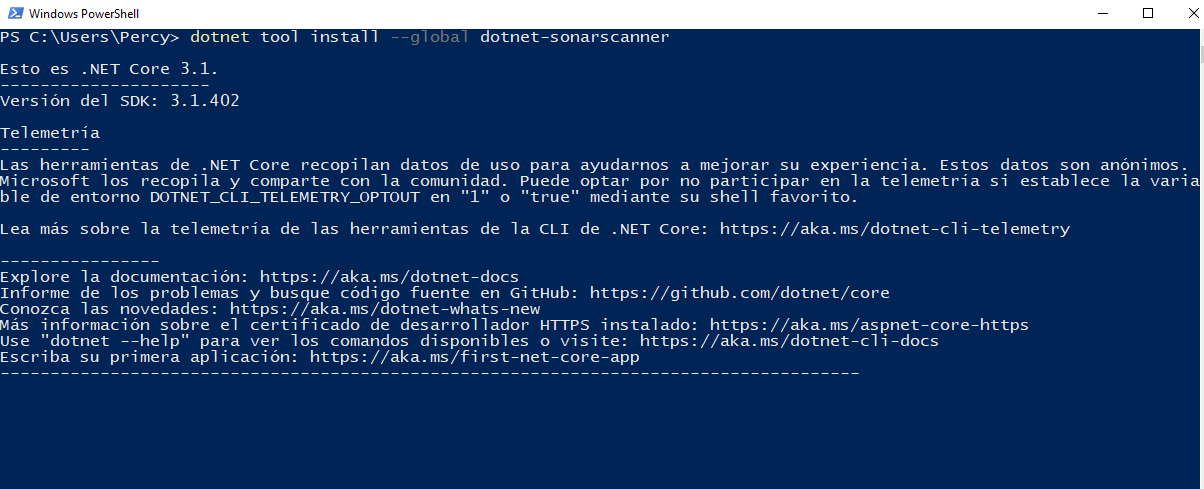
\includegraphics[width=15cm]{./Imagenes/9} 
	\end{center}

\textbf{8. En un terminal, acceder a una ruta donde creara una nueva aplicación}

    \begin{center}
		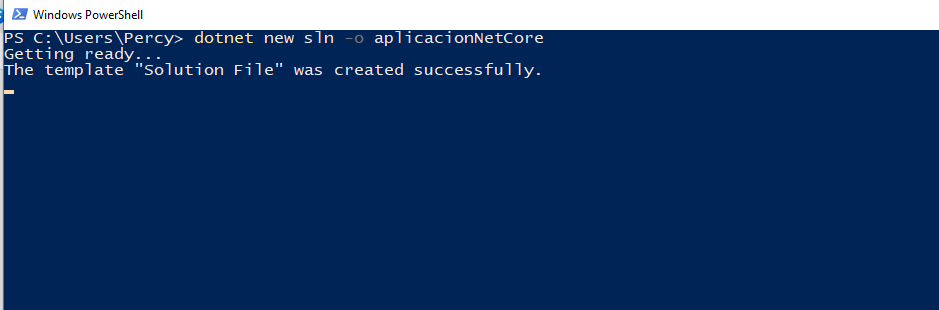
\includegraphics[width=15cm]{./Imagenes/10} 
	\end{center}
	
	 \begin{center}
		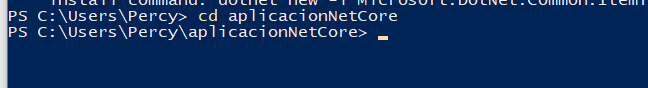
\includegraphics[width=15cm]{./Imagenes/11} 
	\end{center}
	
	 \begin{center}
		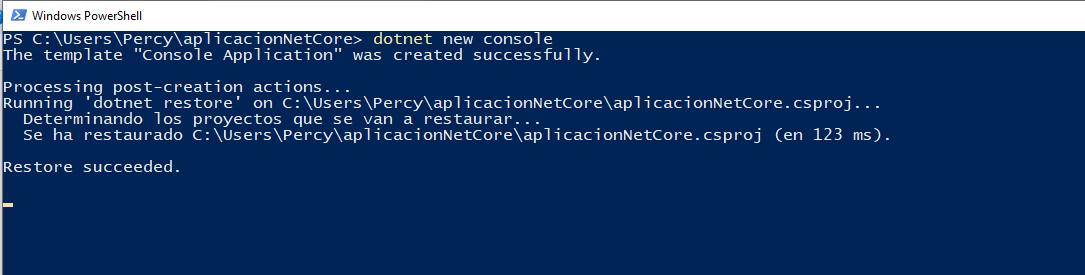
\includegraphics[width=15cm]{./Imagenes/12} 
	\end{center}

	\begin{center}
		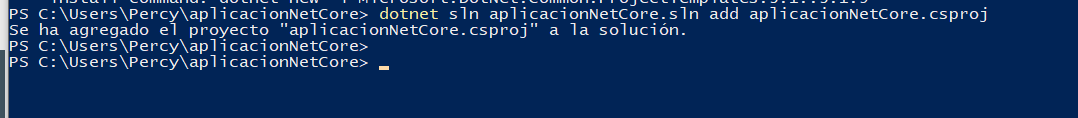
\includegraphics[width=15cm]{./Imagenes/13} 
	\end{center}


\textbf{9. En el mismo terminal, iniciar la sesión de revisión de sonarqube}

   \begin{center}
		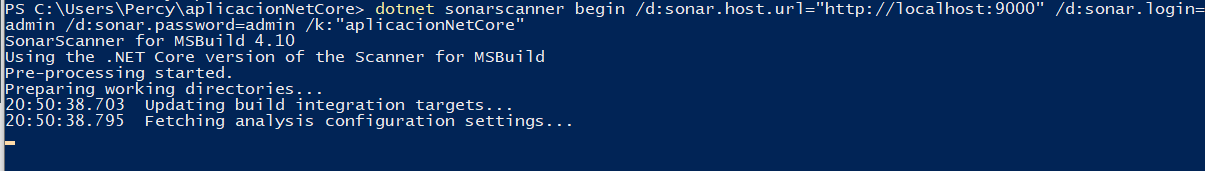
\includegraphics[width=15cm]{./Imagenes/14} 
	\end{center}


\textbf{10. Compilar la aplicación}

    \begin{center}
		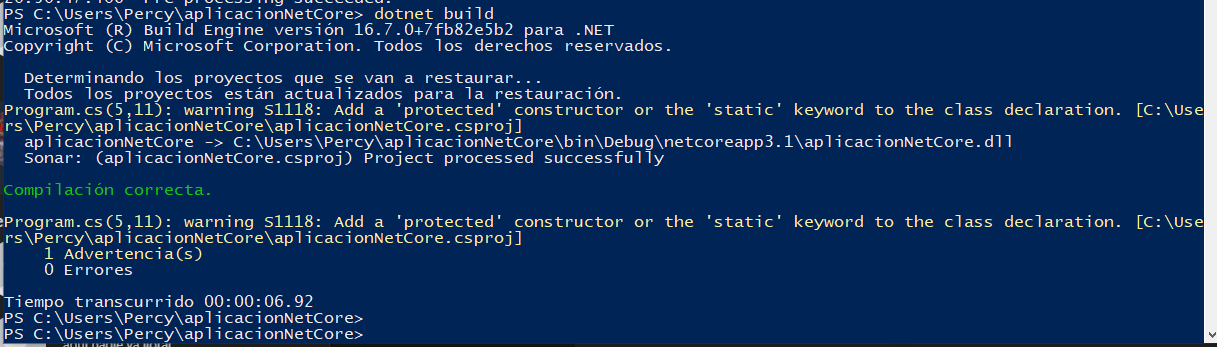
\includegraphics[width=15cm]{./Imagenes/15} 
	\end{center}
	
	
\textbf{11. Cerramos la sesión}

    \begin{center}
		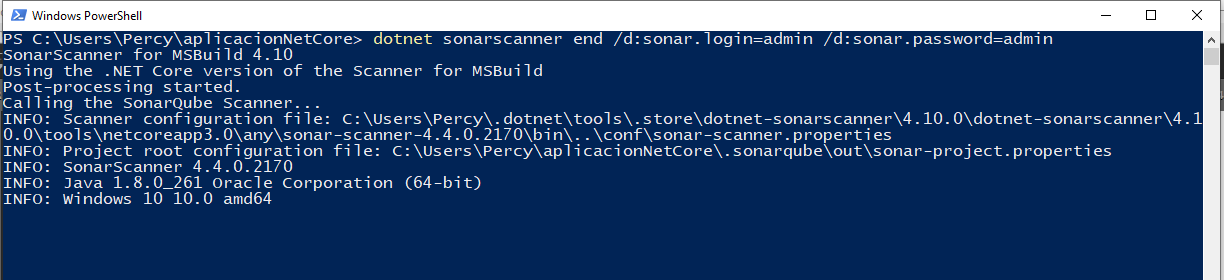
\includegraphics[width=15cm]{./Imagenes/16} 
	\end{center}


   
\end{document}